% Options for packages loaded elsewhere
\PassOptionsToPackage{unicode}{hyperref}
\PassOptionsToPackage{hyphens}{url}
%
\documentclass[
  finnish,
]{book}
\usepackage{lmodern}
\usepackage{amssymb,amsmath}
\usepackage{ifxetex,ifluatex}
\ifnum 0\ifxetex 1\fi\ifluatex 1\fi=0 % if pdftex
  \usepackage[T1]{fontenc}
  \usepackage[utf8]{inputenc}
  \usepackage{textcomp} % provide euro and other symbols
\else % if luatex or xetex
  \usepackage{unicode-math}
  \defaultfontfeatures{Scale=MatchLowercase}
  \defaultfontfeatures[\rmfamily]{Ligatures=TeX,Scale=1}
\fi
% Use upquote if available, for straight quotes in verbatim environments
\IfFileExists{upquote.sty}{\usepackage{upquote}}{}
\IfFileExists{microtype.sty}{% use microtype if available
  \usepackage[]{microtype}
  \UseMicrotypeSet[protrusion]{basicmath} % disable protrusion for tt fonts
}{}
\makeatletter
\@ifundefined{KOMAClassName}{% if non-KOMA class
  \IfFileExists{parskip.sty}{%
    \usepackage{parskip}
  }{% else
    \setlength{\parindent}{0pt}
    \setlength{\parskip}{6pt plus 2pt minus 1pt}}
}{% if KOMA class
  \KOMAoptions{parskip=half}}
\makeatother
\usepackage{xcolor}
\IfFileExists{xurl.sty}{\usepackage{xurl}}{} % add URL line breaks if available
\IfFileExists{bookmark.sty}{\usepackage{bookmark}}{\usepackage{hyperref}}
\hypersetup{
  pdftitle={Bookdown-dokumetti - testi 1},
  pdfauthor={Jussi Hirvonen},
  hidelinks,
  pdfcreator={LaTeX via pandoc}}
\urlstyle{same} % disable monospaced font for URLs
\usepackage{color}
\usepackage{fancyvrb}
\newcommand{\VerbBar}{|}
\newcommand{\VERB}{\Verb[commandchars=\\\{\}]}
\DefineVerbatimEnvironment{Highlighting}{Verbatim}{commandchars=\\\{\}}
% Add ',fontsize=\small' for more characters per line
\usepackage{framed}
\definecolor{shadecolor}{RGB}{248,248,248}
\newenvironment{Shaded}{\begin{snugshade}}{\end{snugshade}}
\newcommand{\AlertTok}[1]{\textcolor[rgb]{0.94,0.16,0.16}{#1}}
\newcommand{\AnnotationTok}[1]{\textcolor[rgb]{0.56,0.35,0.01}{\textbf{\textit{#1}}}}
\newcommand{\AttributeTok}[1]{\textcolor[rgb]{0.77,0.63,0.00}{#1}}
\newcommand{\BaseNTok}[1]{\textcolor[rgb]{0.00,0.00,0.81}{#1}}
\newcommand{\BuiltInTok}[1]{#1}
\newcommand{\CharTok}[1]{\textcolor[rgb]{0.31,0.60,0.02}{#1}}
\newcommand{\CommentTok}[1]{\textcolor[rgb]{0.56,0.35,0.01}{\textit{#1}}}
\newcommand{\CommentVarTok}[1]{\textcolor[rgb]{0.56,0.35,0.01}{\textbf{\textit{#1}}}}
\newcommand{\ConstantTok}[1]{\textcolor[rgb]{0.00,0.00,0.00}{#1}}
\newcommand{\ControlFlowTok}[1]{\textcolor[rgb]{0.13,0.29,0.53}{\textbf{#1}}}
\newcommand{\DataTypeTok}[1]{\textcolor[rgb]{0.13,0.29,0.53}{#1}}
\newcommand{\DecValTok}[1]{\textcolor[rgb]{0.00,0.00,0.81}{#1}}
\newcommand{\DocumentationTok}[1]{\textcolor[rgb]{0.56,0.35,0.01}{\textbf{\textit{#1}}}}
\newcommand{\ErrorTok}[1]{\textcolor[rgb]{0.64,0.00,0.00}{\textbf{#1}}}
\newcommand{\ExtensionTok}[1]{#1}
\newcommand{\FloatTok}[1]{\textcolor[rgb]{0.00,0.00,0.81}{#1}}
\newcommand{\FunctionTok}[1]{\textcolor[rgb]{0.00,0.00,0.00}{#1}}
\newcommand{\ImportTok}[1]{#1}
\newcommand{\InformationTok}[1]{\textcolor[rgb]{0.56,0.35,0.01}{\textbf{\textit{#1}}}}
\newcommand{\KeywordTok}[1]{\textcolor[rgb]{0.13,0.29,0.53}{\textbf{#1}}}
\newcommand{\NormalTok}[1]{#1}
\newcommand{\OperatorTok}[1]{\textcolor[rgb]{0.81,0.36,0.00}{\textbf{#1}}}
\newcommand{\OtherTok}[1]{\textcolor[rgb]{0.56,0.35,0.01}{#1}}
\newcommand{\PreprocessorTok}[1]{\textcolor[rgb]{0.56,0.35,0.01}{\textit{#1}}}
\newcommand{\RegionMarkerTok}[1]{#1}
\newcommand{\SpecialCharTok}[1]{\textcolor[rgb]{0.00,0.00,0.00}{#1}}
\newcommand{\SpecialStringTok}[1]{\textcolor[rgb]{0.31,0.60,0.02}{#1}}
\newcommand{\StringTok}[1]{\textcolor[rgb]{0.31,0.60,0.02}{#1}}
\newcommand{\VariableTok}[1]{\textcolor[rgb]{0.00,0.00,0.00}{#1}}
\newcommand{\VerbatimStringTok}[1]{\textcolor[rgb]{0.31,0.60,0.02}{#1}}
\newcommand{\WarningTok}[1]{\textcolor[rgb]{0.56,0.35,0.01}{\textbf{\textit{#1}}}}
\usepackage{longtable,booktabs}
% Correct order of tables after \paragraph or \subparagraph
\usepackage{etoolbox}
\makeatletter
\patchcmd\longtable{\par}{\if@noskipsec\mbox{}\fi\par}{}{}
\makeatother
% Allow footnotes in longtable head/foot
\IfFileExists{footnotehyper.sty}{\usepackage{footnotehyper}}{\usepackage{footnote}}
\makesavenoteenv{longtable}
\usepackage{graphicx,grffile}
\makeatletter
\def\maxwidth{\ifdim\Gin@nat@width>\linewidth\linewidth\else\Gin@nat@width\fi}
\def\maxheight{\ifdim\Gin@nat@height>\textheight\textheight\else\Gin@nat@height\fi}
\makeatother
% Scale images if necessary, so that they will not overflow the page
% margins by default, and it is still possible to overwrite the defaults
% using explicit options in \includegraphics[width, height, ...]{}
\setkeys{Gin}{width=\maxwidth,height=\maxheight,keepaspectratio}
% Set default figure placement to htbp
\makeatletter
\def\fps@figure{htbp}
\makeatother
\setlength{\emergencystretch}{3em} % prevent overfull lines
\providecommand{\tightlist}{%
  \setlength{\itemsep}{0pt}\setlength{\parskip}{0pt}}
\setcounter{secnumdepth}{5}
\ifxetex
  % Load polyglossia as late as possible: uses bidi with RTL langages (e.g. Hebrew, Arabic)
  \usepackage{polyglossia}
  \setmainlanguage[]{finnish}
\else
  \usepackage[shorthands=off,main=finnish]{babel}
\fi
\usepackage[]{natbib}
\bibliographystyle{apalike}

\title{Bookdown-dokumetti - testi 1}
\author{Jussi Hirvonen}
\date{2020-02-18 (Versio 3.05)}

\begin{document}
\maketitle

{
\setcounter{tocdepth}{1}
\tableofcontents
}
\hypertarget{bookdown-paketin-testidokumentti}{%
\chapter{Bookdown-paketin testidokumentti}\label{bookdown-paketin-testidokumentti}}

Esimerkki Rmarkdownin ja bookdown-paketin käytöstä. Kuvat, taulukot ja kaavat numeroidaan ja niihin voi viitata tekstissä. Lähdeviitteet toimivat, myös ne joissa on ns.

A sample document using RMarkdown with bookdown-package to do statistical analysis and publish a report in html and pdf formats.

\hypertarget{johdanto}{%
\chapter{Johdanto}\label{johdanto}}

\hypertarget{alkutoimia}{%
\section{Alkutoimia}\label{alkutoimia}}

Ero YAML-headerissa lang-parametri (lang: fi). (verrattuna bookdown-demoon).
Bookdown-demossa lisäksi output: pdf\_document, mutta lienee tarpeeton kun kaksi outputformaattia annettu output.yaml-tiedostossa

Bookdown - formaatissa ``juuritiedoston'' indexBD.Rmd tekstit eivät tulostu jos siellä ei ole luvun (chapter) aloittavaa ensimmäisen tason otsikkoa. Siellä on YAML-headeri (metadata).

Lisää YAML-parametreja voi antaa tiedostoissa \_bookdown.yml ja \_output.yml. Nämä lienee välittyvät Pandocille?

Bookdown - demon esimerkkitiedostot ovat nämä:

ouput.yml (huomaa, että \_ - merkki jätetty pois!) (tässä oli bookdown-demo-paketin yml-tiedostot, poistin 3.7.2018)

\hypertarget{tuxe4rkeimmuxe4t-ohjelmistot}{%
\section{Tärkeimmät ohjelmistot}\label{tuxe4rkeimmuxe4t-ohjelmistot}}

\begin{Shaded}
\begin{Highlighting}[]
\KeywordTok{system}\NormalTok{(}\StringTok{"pdflatex --version"}\NormalTok{)}
\end{Highlighting}
\end{Shaded}

\begin{verbatim}
## [1] 0
\end{verbatim}

\begin{Shaded}
\begin{Highlighting}[]
\NormalTok{rmarkdown}\OperatorTok{::}\KeywordTok{pandoc_version}\NormalTok{()}
\end{Highlighting}
\end{Shaded}

\begin{verbatim}
## [1] '2.7.2'
\end{verbatim}

Viimeinen rivi kertoo pandoc-version.
\textbf{20.9.2019} Pandoc-versio tulostuu oikein, mutta pdf-latex - komennon tulosteesta
vain viimeinen rivi. Tässä koko tulos 20.9.2019

MiKTeX-pdfTeX 2.9.7029 (1.40.20) (MiKTeX 2.9.7140 64-bit)

using bzip2 version 1.0.6, 6-Sept-2010

compiled with curl version 7.61.1; using libcurl/7.61.1 WinSSL

compiled with expat version 2.2.6; using expat\_2.2.6

compiled with jpeg version 9.3

compiled with liblzma version 50020042; using 50020042

compiled with libpng version 1.6.35; using 1.6.35

compiled with libressl version LibreSSL 2.8.2; using LibreSSL 2.8.2

compiled with MiKTeX Application Framework version 4.6961; using 4.6961

compiled with MiKTeX Core version 15.7099; using 15.7099

compiled with MiKTeX Archive Extractor version 1.6882; using 1.6882

compiled with MiKTeX Package Manager version 7.7104; using 7.7104

compiled with poppler version 0.60.1

compiled with uriparser version 0.9.2

compiled with zlib version 1.2.11; using 1.2.11

{[}1{]} 0

\hypertarget{muutoksia-tilannetietoja-ja-puutteita}{%
\section{Muutoksia, tilannetietoja ja puutteita}\label{muutoksia-tilannetietoja-ja-puutteita}}

Nyt toimii gitbook \footnote{Virheilmoitukset ovat aika hyödyttömiä. Niiden sijaan tähän alkuun sopisi kuvaus perusideoista ja tekstin muotoiluista. Alaviitteistä esimerkiksi.} ja pdf\_book tulostusformaatteina. Molemmat ovat html-paketteja, ja tarvitsevat ehkä r-datahakemistosta (omalta koneelta) libs-hakemiston jQuery- ja Gitbook-paketit (javaskriptiä ja css-tyylitiedostoja).

test1\_preamble.tex -tiedostoa kokeiltiin, mutta sitä ei saatu heinäkuussa toimimaan.

Lähdeluettelossa Å tulee heti A - kirjaimen jälkeen gitbook-versiossa. PDF-tiedostossa taas Å-alkuinen sukunimi sijoittuu vähän toisin virheellisesti. Ikävä juttu!

\hypertarget{voiko-rmd-dokumentin-ensimmuxe4iselluxe4-rivilluxe4-olla-toisen-tason-otsikko}{%
\chapter{Voiko rmd-dokumentin ensimmäisellä rivillä olla toisen tason otsikko?}\label{voiko-rmd-dokumentin-ensimmuxe4iselluxe4-rivilluxe4-olla-toisen-tason-otsikko}}

Lisätään tiedosto 011-test\_johd.Rmd, ja katsotaan toimiiko. Tämä helpottaisi
isomman dokumentin rakentamista. Tässä Bookdown kokoaa tiedostot ``aakkosjärjestyksessä'',
mutta ne voi myös luetella eksplisiittisesti bookdown.yml -tiedostossa.

``Warning \url{message:In} split\_chapters(output, gitbook\_page, number\_sections, split\_by, :
You have 7 Rmd input file(s) but only 6 first-level heading(s). Did you forget first-level headings in certain Rmd files?''

Mutta näyttäisi toimivan, jätetään kuitenkin pois (13.7.2019). Voi aiheuttaa hämminkiä viitteissä, sisällysluettelossa ja muussakin.

\hypertarget{kaavat-ja-matemattiset-merkinnuxe4t}{%
\chapter{Kaavat ja matemattiset merkinnät}\label{kaavat-ja-matemattiset-merkinnuxe4t}}

Kaavat on esitettävä bookdown-paketin määrityksillä. Viittausnimien on oltava yksikäsitteisiä koko dokumentissa, jos käytetään ``merge and knit'' menetelmää. Jos taas jokainen lapsidokumentti on ``itsenäinen'' (``knit and merge''), tämä koskee vain kyseistä dokumenttia (kts. Bookdown - webkirja).

Kaavoissa iso ongelma heinäkuussa oli tämä:

\textbf{equation-tägien välissä ei saa olla tyhjiä rivejä!}

\hypertarget{kahden-luokittelumuuttuja-taulukko}{%
\section{Kahden luokittelumuuttuja taulukko}\label{kahden-luokittelumuuttuja-taulukko}}

Kahden luokittelumuuttujan riippuvuutta voidaan testata \(\chi^{2}\) - testillä. Testisuure saadaan laskemalla yhteen jokaisen solun havaittujen ja odotetettujen (riippumattomuushypoteesi) frekvenssien erotukset muodossa

\begin{equation}
  \chi^{2} = \frac{(havaittu - odotettu)^2} {odotettu}
  \label{eq:khii21}
\end{equation}

Tämä voidaan esittää ca:han sopivammalla tavalla parilla muunnoksella, jolloin saamme riveittäin vastaavat termit rivisummalla painotettuna:

\begin{equation}
  rivisumma \times \frac{(havaittu \: riviprofiili - odotettu \: riviprofiili)^2} {odotettu \: riviprofiili}
  \label{eq:khii22}
\end{equation}

Kun jaamme nämä tekijät havaintojen kokonaismäärällä \(n\), rivisumma muuntuu rivin massaksi, ja niiden summa muotoon \(\frac{\chi^{2}}{n}\).

\begin{equation}
 \frac{\chi^{2}}{n} = \phi^{2}
 \label{eq:inert1}
\end{equation}

Tunnusluku \(\phi^{2}\) on korrespondenssianalyysissä kokonaisinertia (total inertia). Se kuvaa, kuinka paljon varianssia taulukossa on ja on riippumaton havaintojen lukumäärästä. Tilastotieteessä tunnusluvulla on useita vaihtoehtoisia nimiä (esim. mean square contingency coefficient), ja sen neliöjuurta kutsutaan \(\phi\) - kertoimeksi.

Tässä siirrytään kahden luokittelumuuttujan taulukosta suhteellisten frekvenssien taulukkoon, ja pieni pohdinta taulukoista yleensä olisi paikallaan. Yhtälöihin voi viitata \eqref{eq:khii21} . Kokeillaan vielä, toimivatko kirjallisuusviittet, kuten tärkeä lähde\citep{RefWorks:55}.

\hypertarget{taulukot-ja-kuvat}{%
\chapter{Taulukot ja kuvat}\label{taulukot-ja-kuvat}}

Tähän taulukoita ja kuvia, esimerkkiaineistoilla.

Kirjallisuutta on myös \citep{RefWorks:68}, ja \citep{RefWorks:57} esittelee geometrisen tulkinnan peruskäsitteet yksinkertaisen kahden luokittelumuuttujan korrespondenssianalyysin avaulla. Mitenköhän skandit toimivat lähteissä, bib-tiedostossa on niitä myös escape-muodossa (katso esim. \citep{RefWorks:100}, kritiikkiä on esittänyt \citep{RefWorks:110})

Viitteet saa tulostusasetuksilla yhdelle sivulle, oletuksena on viitteiden esittäminen jokaisen sivun alareunassa.

\hypertarget{taulukoita}{%
\section{Taulukoita}\label{taulukoita}}

Tästä poistettu koodilohko data\_1, ei tarvita jos ca-paketti on ladattu. Ja alaviiva on aikanakin ref-labeleissa kielletty. Koodilohkojen nimissä taitaa olla sallittu?

Taulukot tulostetaan funktiolla knitr::kable(). Taulukko numeroidaan ja se saa automaattisesti labelin etutunnisteella `tab', ja siihen liitetään chunk-label (esim alla tab:smoketable1).

Tämä koodipätkä ei antaa yhden kappaleen esikatselussa virheilmoituksen, ``smoke''-dataa ei löydy.

\begin{Shaded}
\begin{Highlighting}[]
\NormalTok{knitr}\OperatorTok{::}\KeywordTok{kable}\NormalTok{(smoke[,}\DecValTok{1}\OperatorTok{:}\DecValTok{4}\NormalTok{], }\DataTypeTok{booktabs =} \OtherTok{TRUE}\NormalTok{,}
  \DataTypeTok{caption =} \StringTok{'CA-paketin smoke-data (keinotekoinen)'}
\NormalTok{)}
\end{Highlighting}
\end{Shaded}

\begin{table}

\caption{\label{tab:smoketable1}CA-paketin smoke-data (keinotekoinen)}
\centering
\begin{tabular}[t]{lrrrr}
\toprule
  & none & light & medium & heavy\\
\midrule
SM & 4 & 2 & 3 & 2\\
JM & 4 & 3 & 7 & 4\\
SE & 25 & 10 & 12 & 4\\
JE & 18 & 24 & 33 & 13\\
SC & 10 & 6 & 7 & 2\\
\bottomrule
\end{tabular}
\end{table}

\begin{Shaded}
\begin{Highlighting}[]
\CommentTok{# Taulukkoon viittaaminen tekstissä \textbackslash{}@ref(label)}
\end{Highlighting}
\end{Shaded}

Taulukossa \ref{tab:smoketable1} on kahden luokittelumuuttujan keinotekoinen esimerkkiaineisto tupakonnin määrästä henkilöstöryhmittäin (SM = senior managemet, JM = junior management, SE ja JE vastaavasti ryhmälle employee, SC = secretary).

Useampi taulukko saadaan taulukkoympäristöön (table environment) yhdistämällä data-objektit listaksi.

\begin{Shaded}
\begin{Highlighting}[]
\CommentTok{# riviprofiilit}
\NormalTok{smoke.rpro <-}\StringTok{ }\NormalTok{smoke }\OperatorTok{/}\StringTok{ }\KeywordTok{rowSums}\NormalTok{ (smoke)}
\CommentTok{# keskiarvoprofiili}
\NormalTok{smoke.avrpro <-}\StringTok{ }\KeywordTok{colSums}\NormalTok{(smoke) }\OperatorTok{/}\StringTok{ }\KeywordTok{sum}\NormalTok{(smoke)}

\NormalTok{knitr}\OperatorTok{::}\KeywordTok{kable}\NormalTok{(}
  \KeywordTok{list}\NormalTok{(smoke.rpro, }\KeywordTok{t}\NormalTok{(smoke.avrpro)   ), }\DataTypeTok{digits =} \DecValTok{3}\NormalTok{,}
  \DataTypeTok{caption =} \StringTok{'Riviprofiilit ja keskiarvoprofiili'}\NormalTok{, }\DataTypeTok{booktabs =} \OtherTok{TRUE}
\NormalTok{)}
\end{Highlighting}
\end{Shaded}

\begin{table}
\caption{\label{tab:smoketable2}Riviprofiilit ja keskiarvoprofiili}

\centering
\begin{tabular}[t]{lrrrr}
\toprule
  & none & light & medium & heavy\\
\midrule
SM & 0.364 & 0.182 & 0.273 & 0.182\\
JM & 0.222 & 0.167 & 0.389 & 0.222\\
SE & 0.490 & 0.196 & 0.235 & 0.078\\
JE & 0.205 & 0.273 & 0.375 & 0.148\\
SC & 0.400 & 0.240 & 0.280 & 0.080\\
\bottomrule
\end{tabular}
\centering
\begin{tabular}[t]{rrrr}
\toprule
none & light & medium & heavy\\
\midrule
0.316 & 0.233 & 0.321 & 0.13\\
\bottomrule
\end{tabular}
\end{table}

Taulukossa \ref{tab:smoketable2} on laskettu jokaisen rivin riviprofiilit. Ne saadan kun rivin luvut jaetaan rivin summalla. Yhden rivin taulukossa on esitetty riviprofiilien keskikarvo, sarakesummat jaettuna koko taulukon havaintojen lukumäärällä. Sen prosenttiluvut kertovat tupakoititapojen jakauman koko henkilöstössä.

Jos PDF-tulostuksessa ei haluta ns. kelluvaa taulukkoa (float), voi kable-funktiossa käyttää LaTeXin pakettia longtable. Silloin on myös muistettava ottaa paketti käyttöön (usepackage\{\}) LaTeX - pohjatiedostossa (preamble).

Pandoc tukee monia Markdownin taulukkotyyppejä. Viittaaminen vaaati labeloidun otsikon, ja sen on oltava otsikkotestin alussa määrämuotoisena (esim. ab:hienotaulu). Tämä vaatii tarkkuutta, jos taulukon pitää toimia html- ja LaTex-outputissa. kable-funktiota kannattaa käyttää!

\hypertarget{korrespondenssianalyysin-numeeriset-tulokset-taulukoina}{%
\section{Korrespondenssianalyysin numeeriset tulokset taulukoina}\label{korrespondenssianalyysin-numeeriset-tulokset-taulukoina}}

Korrespondenssianalyysin idea on vähentää aineiston dimensioita, ja esittää taulukon rivien ja sarakkeiden riippuvuudet yleensä kaksiulotteisena karttana.

Numeeriset tulokset ovat tärkeitä diagnostiikassa ja kartan laadun varmistuksessa. Niistä näkee myös täsmällisesti, mitkä rivit ja sarakkeet määrittävät koordinaatiston.

\begin{Shaded}
\begin{Highlighting}[]
\NormalTok{smokeCA <-}\StringTok{ }\KeywordTok{ca}\NormalTok{(smoke)}
\CommentTok{#temp1 <- smokeCA tämä kai tarpeeton ? (4.12.2018)}
\NormalTok{numres1CA1 <-}\StringTok{ }\KeywordTok{summary}\NormalTok{(smokeCA)}
\CommentTok{#str(smokeCA)}
\CommentTok{#knitr::kable( smokeCA,}
\CommentTok{#  digits = 3,}
\CommentTok{#  caption = 'Riviprofiilit ja keskiarvoprofiili', booktabs = TRUE}
\CommentTok{#)}
\CommentTok{#str(temp1)}
\CommentTok{#stargazer(temp2$rows, type = "text", title = "CA-tuloksia")}
\CommentTok{# LateX-tulostuksessa float vaatii jotain tällaista:Table: (\textbackslash{}#tab:cataul1) }
\CommentTok{#str(temp2)}
\CommentTok{#str(temp2$scree)}
\CommentTok{#temp2$scree}
\NormalTok{numres1CA1}
\end{Highlighting}
\end{Shaded}

\begin{verbatim}
## 
## Principal inertias (eigenvalues):
## 
##  dim    value      %   cum%   scree plot               
##  1      0.074759  87.8  87.8  **********************   
##  2      0.010017  11.8  99.5  ***                      
##  3      0.000414   0.5 100.0                           
##         -------- -----                                 
##  Total: 0.085190 100.0                                 
## 
## 
## Rows:
##     name   mass  qlt  inr    k=1 cor ctr    k=2 cor ctr  
## 1 |   SM |   57  893   31 |  -66  92   3 | -194 800 214 |
## 2 |   JM |   93  991  139 |  259 526  84 | -243 465 551 |
## 3 |   SE |  264 1000  450 | -381 999 512 |  -11   1   3 |
## 4 |   JE |  456 1000  308 |  233 942 331 |   58  58 152 |
## 5 |   SC |  130  999   71 | -201 865  70 |   79 133  81 |
## 
## Columns:
##     name   mass  qlt  inr    k=1 cor ctr    k=2 cor ctr  
## 1 | none |  316 1000  577 | -393 994 654 |  -30   6  29 |
## 2 | lght |  233  984   83 |   99 327  31 |  141 657 463 |
## 3 | medm |  321  983  148 |  196 982 166 |    7   1   2 |
## 4 | hevy |  130  995  192 |  294 684 150 | -198 310 506 |
\end{verbatim}

Taulukot ovatkin aika vaikeita, tulostiedoista! Stargazer toki tekee monenlaista, mutta kun kyse on hyvin yksinkertaisista tulostaulukoista kablen pitäisi toimia.

Kokeillaan summary(smokeCA) - listan dataframe-olioden tulostusta kablella. Voisi harkita funktiota, joka poimii CA:n tuloslistasta sopivat objektit kable-funktiolle? Stargazer taas vaatisi (luultavasti) jonkun ehdollisen tulostuksen (PDF ja html)?

\begin{Shaded}
\begin{Highlighting}[]
\NormalTok{knitr}\OperatorTok{::}\KeywordTok{kable}\NormalTok{( numres1CA1}\OperatorTok{$}\NormalTok{rows,}
    \DataTypeTok{digits =} \DecValTok{3}\NormalTok{,          }
    \DataTypeTok{caption =} \StringTok{'Korrespondenssianalyysin diagnostiikkaa - rivit'}\NormalTok{, }\DataTypeTok{booktabs =} \OtherTok{TRUE}
\NormalTok{)}
\end{Highlighting}
\end{Shaded}

\begin{table}

\caption{\label{tab:simpleCAtab1}Korrespondenssianalyysin diagnostiikkaa - rivit}
\centering
\begin{tabular}[t]{lrrrrrrrrr}
\toprule
name & mass &  qlt &  inr &  k=1 & cor & ctr &  k=2 & cor & ctr\\
\midrule
SM & 57 & 893 & 31 & -66 & 92 & 3 & -194 & 800 & 214\\
JM & 93 & 991 & 139 & 259 & 526 & 84 & -243 & 465 & 551\\
SE & 264 & 1000 & 450 & -381 & 999 & 512 & -11 & 1 & 3\\
JE & 456 & 1000 & 308 & 233 & 942 & 331 & 58 & 58 & 152\\
SC & 130 & 999 & 71 & -201 & 865 & 70 & 79 & 133 & 81\\
\bottomrule
\end{tabular}
\end{table}

Rivien ja sarakkeiden diagnotiikkataulukot eivät mahdu rinnakkain, siksi ne tulostetaan erikseen.

\begin{Shaded}
\begin{Highlighting}[]
\NormalTok{knitr}\OperatorTok{::}\KeywordTok{kable}\NormalTok{( numres1CA1}\OperatorTok{$}\NormalTok{columns,}
    \DataTypeTok{digits =} \DecValTok{3}\NormalTok{,          }
    \DataTypeTok{caption =} \StringTok{'Korrespondenssianalyysin diagnostiikkaa - sarakkeet'}\NormalTok{, }\DataTypeTok{booktabs =} \OtherTok{TRUE}
\NormalTok{)}
\end{Highlighting}
\end{Shaded}

\begin{table}

\caption{\label{tab:simpleCAtab2}Korrespondenssianalyysin diagnostiikkaa - sarakkeet}
\centering
\begin{tabular}[t]{lrrrrrrrrr}
\toprule
name & mass &  qlt &  inr &  k=1 & cor & ctr &  k=2 & cor & ctr\\
\midrule
none & 316 & 1000 & 577 & -393 & 994 & 654 & -30 & 6 & 29\\
lght & 233 & 984 & 83 & 99 & 327 & 31 & 141 & 657 & 463\\
medm & 321 & 983 & 148 & 196 & 982 & 166 & 7 & 1 & 2\\
hevy & 130 & 995 & 192 & 294 & 684 & 150 & -198 & 310 & 506\\
\bottomrule
\end{tabular}
\end{table}

Taulukoiden \ref{tab:simpleCAtab1} ja \ref{tab:simpleCAtab2} luvut on kerrottu tuhannella (``per milles'').

Dimensioiden ominaisarvot (eli niiden osuus kokonaisinertiasta) saadaan ca-funktion tuloslistasta taulukoksi. Se esitetään joskus myös ns. scree - kuvana, jos dimensoita on paljon ja joudutaan pohtimaan kuinka monta valitaan (vaikea kysymys!).

\begin{Shaded}
\begin{Highlighting}[]
\NormalTok{knitr}\OperatorTok{::}\KeywordTok{kable}\NormalTok{( numres1CA1}\OperatorTok{$}\NormalTok{scree,}
    \DataTypeTok{digits =} \DecValTok{3}\NormalTok{,          }
    \DataTypeTok{caption =} \StringTok{'Korrespondenssianalyysin diagnostiikkaa - ominaisarvot'}\NormalTok{, }\DataTypeTok{booktabs =} \OtherTok{TRUE}
\NormalTok{)}
\end{Highlighting}
\end{Shaded}

\begin{table}

\caption{\label{tab:simpleCAscree}Korrespondenssianalyysin diagnostiikkaa - ominaisarvot}
\centering
\begin{tabular}[t]{rrrr}
\toprule
 & values & values2 & values3\\
\midrule
1 & 0.075 & 87.756 & 87.756\\
2 & 0.010 & 11.759 & 99.515\\
3 & 0.000 & 0.485 & 100.000\\
\bottomrule
\end{tabular}
\end{table}

Taulukko \ref{tab:simpleCAscree} vaatii selityksen, mutta kuvaa ei tässä tapauksessa tarvita.

\hypertarget{kuvat}{%
\section{Kuvat}\label{kuvat}}

\textbf{chunk-optiot}

fig.cap: R plot - kuvat figure-ympäristöön, automaattiset labelit (fig: + koodipätkän label) ja niihin voi viitata.

fig.asp oikeaan arvoon 1.

\begin{Shaded}
\begin{Highlighting}[]
\KeywordTok{plot}\NormalTok{(smokeCA)}
\end{Highlighting}
\end{Shaded}

\begin{figure}
\centering
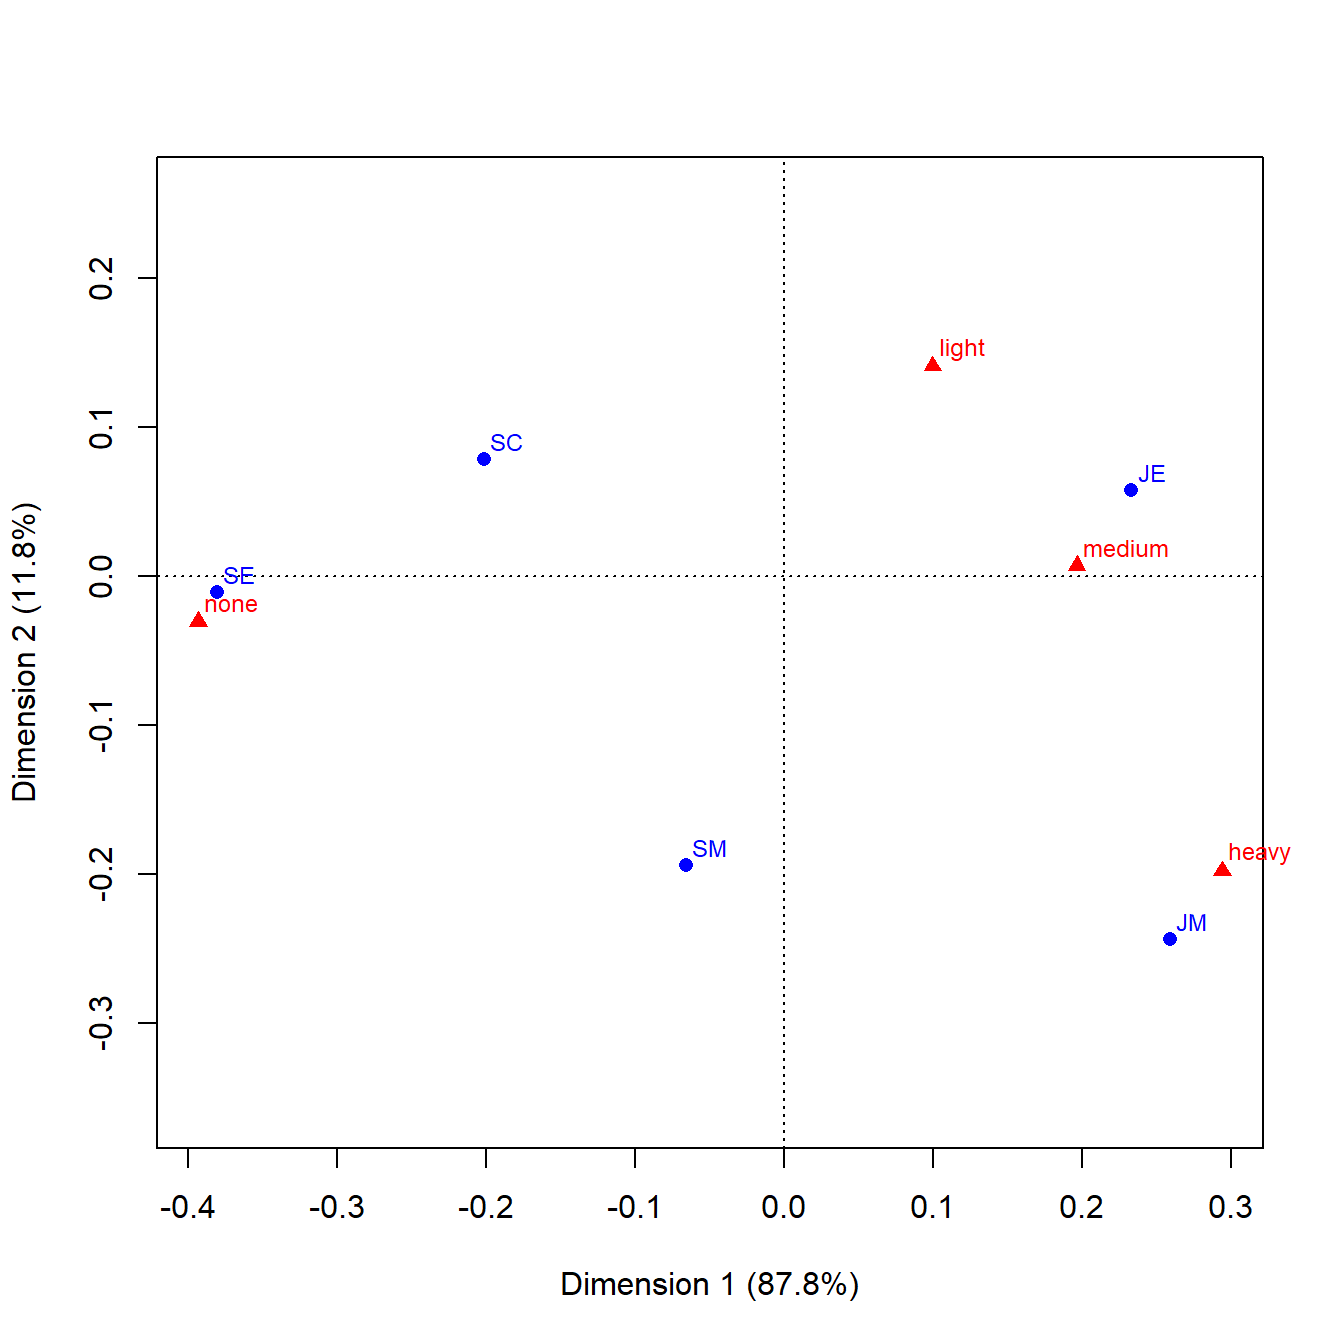
\includegraphics{bookdown-testi1_files/figure-latex/CAmap1-1.pdf}
\caption{\label{fig:CAmap1}CA-kartta}
\end{figure}

Kuviin (kuten \ref{fig:CAmap1}) ja taulukoihin voi viitata tekstissä. Kuvan otsikko tulostuu kuvan alapuolelle, ehkä vähän huono idea?

Näköjään stargazer-kokeilu tulostusoptiolla ``html'' loi R-projektihakemistoon kansion ja sinne png-kuvan.
finnish.ldf tiedoston muokkaus MikTeX:ssä tehty, mutta se ei vaikuta html-viiteotsikkoon. Korjattu ``ehdollisessa viitesivussa'' viitteet.Rmd jossa html-viiteluettelon otsikko annetaan.

Saisiko numeeristen tulosten scree-kuvan samalla tavalla kuvaksi?

\hypertarget{bookdown-ja-rmarkdown}{%
\chapter{Bookdown ja Rmarkdown}\label{bookdown-ja-rmarkdown}}

Bookdown- R-paketti ``paketoi'' RMarkdownin tulostutoiminnot (output) ja sen monet säädettävät optiot. Samat Rmd-dokumentit saadaan koottua moneen eri formaattiin: html- sivuiksi, PDF-dokumentiksi tai Ebook-kirjaksi. Kaikissa tulostusvaihtoehdoissa on monia eri vaihtoehtoja. Html-tulostuksessa voi valita yhden tai useamman html-sivun lisäksi gitbook- tai Tufte- vaihtoehdon. Ne on toteutettu css-tyylitiedostoilla ja JavaScript-kirjastoilla. Tässä on käytetty gitbook-formaattia.

LaTeX-formaatti renderöidään jollain LaTeX-vaihtoehdolla PDF-tiedostoksi. \textbf{ToDo} PDF-formaattejakin on useita variantteja, mikä niistä. Tässä vaihtoehdossa konfigurointimahdollisuudet ovat käytännössä rajattomat, sillä välitulosteena syntyvää TeX-tiedostoa voi muokata ja muuntaa sen sitten PDF-muotoon.

Prosessissa on monta vaihtetta, ja eri parametrien yhteisvaikutusta on vaikea hahmottaa.

\begin{Shaded}
\begin{Highlighting}[]
\NormalTok{knitr}\OperatorTok{::}\KeywordTok{include_graphics}\NormalTok{(}\StringTok{'BookdownProc.png'}\NormalTok{)}
\end{Highlighting}
\end{Shaded}

\begin{figure}

{\centering 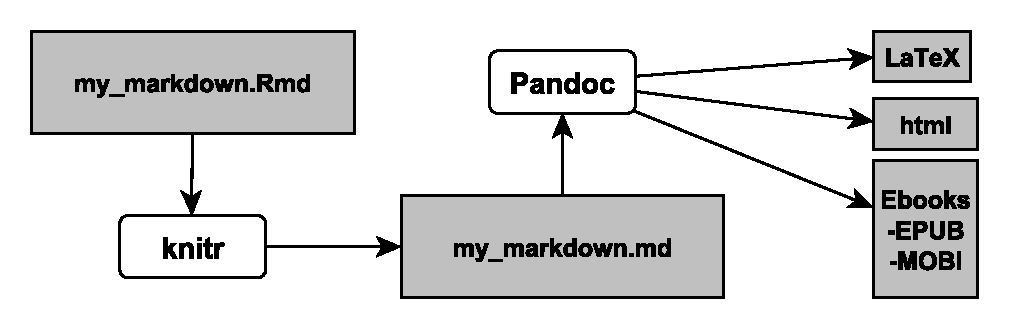
\includegraphics[width=0.5\linewidth]{BookdownProc} 

}

\caption{Tulostiedoston prosessointi - png}\label{fig:bdprocess1}
\end{figure}

Perusopas bookdown paketin käyttöön on Yihui Xien \href{https://bookdown.org/yihui/bookdown/}{``bookdown: Authoring Books and Technical Documents with R Markdown''"}. Siinä pääidea on tuottaa yhdellä Rmd-koodilla kuvan
\ref{fig:bdprocess1} kolme vaihtoehtoista tulostiedostoa mahdollisimman yksinkertaisesti. Knitr- ohjelma ``kutoo'' Rmd-tiedoston r-koodilohkojen tulokset ja tekstin markdown-tiedostoksi (md). Rmd-tiedostojen YAML-asetukset siirtyvät Pandocille, joka täydentää niillä omia mallitiedostojaan (template).

Asetuksia on useammassa paikassa. YAML- asetuksista bd-kirja kertoo näin: ''More bookdown configuration options in \_bookdown.yml are explained in Section 4.4. Besides these configurations, you can also specify some Pandoc-related configurations in the YAML metadata of the first Rmd file of the book, such as the title, author, and date of the book, etc.'' Tärkeintä on yksikertaisuus, lopullista ulkoasua voi hioa kun kokonaisuus on valmis.

Laajempi ja tarkempi opas ilmestyi 15.7.2018, kolmen kirjoittajan \href{https://bookdown.org/yihui/rmarkdown/}{``R Markdown: The Definitive Guide''}. Siinä eri asetusten hierarkia on kuvattu tarkemmin ja selkeämmin. Tulostusvaihtoehtoja esitellään laajemmin, bookdown on vain yksi luku.

R Studiolla alkuun pääse helposti, kun lataa bookdown-paketin, ja luo uuden bookdown-projektin. Xien ensimmäisen kirjan alku-luvut ja uudemman teoksen johdattelut auttavat jatkoon.

\textbf{Käytännön vinkkejä}

\begin{enumerate}
\def\labelenumi{\arabic{enumi}.}
\item
  Kuvasuhde pitää olla 1:1 . Ehkä hankalin juttu Rmarkdownin kanssa työskennellessä, mutta aina voi avata oman grafiikkaikkunan. Dataa analysoidessa voi tallentaa kuvat pdf-muodossa, lisäillä kommentteja yms. Lopullisessa dokumentissa kuvasuhden pitää erikseen tarkista, säätämiseen on monta vipua.
\item
  Bookdown-työskentelyssä pdf-tuloste ei ole kätevä, yleensä analyysiä hiotaan Rmd-tiedosto kerrallaan. R Studio voi yllättää aina joskus! Knit-napin takaa löytyy kuitenkin eri renderöintifuktiot kuin oikean laidan yläikkunan ``Build Book'' - valikosta. Knitr-funktiota kannattaa käyttää, jos haluaa katsoa yhden Rmd-tiedoston tulostetta. Tarkista kuitenkin, että (a) Rmd-tiedostoon ei automaattisesti lisäillä YAML-headereita ja (b) projektin hakemistoon ei ilmesty ylimääräisiä Rmd-tiedostoja. Joskus bookdown R Studion kanssa kasaa yhden Rmd-tiedoston tulostuksessa ``väliaikaiseksi'' tiedostoksi koko dokumentin yhteen .Rmd -tiedostoon. Jos bookdown-projektiin kuuluvia Rmd-tiedostoja ei eksplitsiittisesti luetella (suositeltavaa, laita bookdown.yml - tiedostoon lista) syntyy hassua sotkua.
\item
  Koko raportin tulostus html-muodossa käy kätevimmin ``Build book'' - valikon html-book- funktiolla/formaatilla. Tämä pitää tsekata! (4.12.18)
\item
  Suositus: koko dokumentit tulostukset aina ``puhtaalta pöydältä'', käynnistä R uudelleen. Myös silloin, kun tulostat ensin vaikka gitbookin ja sitten pdf-tiedoston.
\end{enumerate}

Windows-ympäristössä (Windows 10) MikTeXin kanssa voi tulla ongelmia, jos käytät konetta tavallisen käyttäjän oikeuksilla. Bookdown-paketin kanssa on kätevää käyttää tinytex - r-pakettia, ja konfiguroida oman koneen MikTeX - asennus asentamaan tarvittavat paketit ``lennossa''. Peruskäyttäjän omat paketit voivat vaatia päivitystä, mutta oikeudet eivät riitä. Pulman voi ratkaista, kun käynnistää MikTeXin paketinhallintasovelluksen (jolla on monta nimeä, admin console jne) peruskäyttäjänä, ja katsoo mitä päivityksiä on tarjolla. Nämä paketit voi sitten asentaa admin-oikeuksilla.

Kokeillaan vielä PDF-kuvan liittämistä dokumenttiin. Ei näy html-tulosteessa.

\begin{Shaded}
\begin{Highlighting}[]
\NormalTok{knitr}\OperatorTok{::}\KeywordTok{include_graphics}\NormalTok{(}\StringTok{'BookdownProc.pdf'}\NormalTok{)}
\end{Highlighting}
\end{Shaded}

\begin{figure}

{\centering 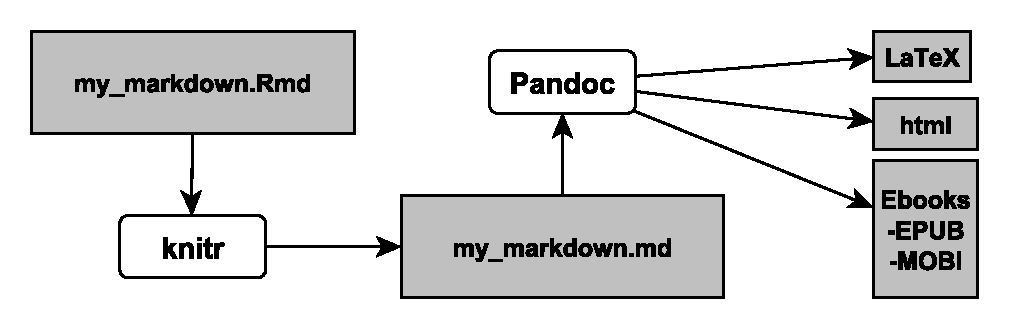
\includegraphics[width=0.5\linewidth]{BookdownProc} 

}

\caption{Tulostiedoston prosessointi - pdf}\label{fig:bdprocess2}
\end{figure}

Testataan koodilohkojen listausta, näyttää toimivan mutta vaatii vielä säätämistä. Ohje löytyi \href{https://yihui.name/en/2018/09/code-appendix/}{Yihui Xienin blogista} (luettu 26.10.2018).

\begin{Shaded}
\begin{Highlighting}[]
\CommentTok{# pitääkö kirjastot ladata tässä, vai jokaisen rmd-tiedoston alussa? library(rgl)}
\KeywordTok{library}\NormalTok{(ca)}
\KeywordTok{library}\NormalTok{(rgl) }\CommentTok{# ongelmia jossain vaiheessa, kokeillaan toimiiko nyt (18.2.20)}
\KeywordTok{library}\NormalTok{(haven)}
\KeywordTok{library}\NormalTok{(dplyr)}
\KeywordTok{library}\NormalTok{(knitr)}
\KeywordTok{library}\NormalTok{(tidyverse)}
\KeywordTok{library}\NormalTok{(lubridate)}
\KeywordTok{library}\NormalTok{(rmarkdown)}
\KeywordTok{library}\NormalTok{(ggplot2)}
\KeywordTok{library}\NormalTok{(furniture)}
\KeywordTok{library}\NormalTok{(likert)}
\KeywordTok{library}\NormalTok{(scales) }\CommentTok{# G_1_2 - kuva}
\KeywordTok{library}\NormalTok{(reshape2)  }\CommentTok{# G_1_2 - kuva}
\KeywordTok{library}\NormalTok{(printr) }\CommentTok{#19.5.18 taulukoiden ja matriisien tulostukseen - onkohan tarpeen? (29.6.2019)}
\KeywordTok{library}\NormalTok{(stargazer) }\CommentTok{# 28.5.2018, ei käytetet joten pois (18.2.20)}
\KeywordTok{library}\NormalTok{(bookdown)}
\KeywordTok{library}\NormalTok{(tinytex)}
\KeywordTok{system}\NormalTok{(}\StringTok{"pdflatex --version"}\NormalTok{)}
\NormalTok{rmarkdown}\OperatorTok{::}\KeywordTok{pandoc_version}\NormalTok{()}


\NormalTok{knitr}\OperatorTok{::}\KeywordTok{kable}\NormalTok{(smoke[,}\DecValTok{1}\OperatorTok{:}\DecValTok{4}\NormalTok{], }\DataTypeTok{booktabs =} \OtherTok{TRUE}\NormalTok{,}
  \DataTypeTok{caption =} \StringTok{'CA-paketin smoke-data (keinotekoinen)'}
\NormalTok{)}
\CommentTok{# Taulukkoon viittaaminen tekstissä \textbackslash{}@ref(label)}
\CommentTok{# riviprofiilit}
\NormalTok{smoke.rpro <-}\StringTok{ }\NormalTok{smoke }\OperatorTok{/}\StringTok{ }\KeywordTok{rowSums}\NormalTok{ (smoke)}
\CommentTok{# keskiarvoprofiili}
\NormalTok{smoke.avrpro <-}\StringTok{ }\KeywordTok{colSums}\NormalTok{(smoke) }\OperatorTok{/}\StringTok{ }\KeywordTok{sum}\NormalTok{(smoke)}

\NormalTok{knitr}\OperatorTok{::}\KeywordTok{kable}\NormalTok{(}
  \KeywordTok{list}\NormalTok{(smoke.rpro, }\KeywordTok{t}\NormalTok{(smoke.avrpro)   ), }\DataTypeTok{digits =} \DecValTok{3}\NormalTok{,}
  \DataTypeTok{caption =} \StringTok{'Riviprofiilit ja keskiarvoprofiili'}\NormalTok{, }\DataTypeTok{booktabs =} \OtherTok{TRUE}
\NormalTok{)}

\NormalTok{smokeCA <-}\StringTok{ }\KeywordTok{ca}\NormalTok{(smoke)}
\CommentTok{#temp1 <- smokeCA tämä kai tarpeeton ? (4.12.2018)}
\NormalTok{numres1CA1 <-}\StringTok{ }\KeywordTok{summary}\NormalTok{(smokeCA)}
\CommentTok{#str(smokeCA)}
\CommentTok{#knitr::kable( smokeCA,}
\CommentTok{#  digits = 3,}
\CommentTok{#  caption = 'Riviprofiilit ja keskiarvoprofiili', booktabs = TRUE}
\CommentTok{#)}
\CommentTok{#str(temp1)}
\CommentTok{#stargazer(temp2$rows, type = "text", title = "CA-tuloksia")}
\CommentTok{# LateX-tulostuksessa float vaatii jotain tällaista:Table: (\textbackslash{}#tab:cataul1) }
\CommentTok{#str(temp2)}
\CommentTok{#str(temp2$scree)}
\CommentTok{#temp2$scree}
\NormalTok{numres1CA1}

\NormalTok{knitr}\OperatorTok{::}\KeywordTok{kable}\NormalTok{( numres1CA1}\OperatorTok{$}\NormalTok{rows,}
    \DataTypeTok{digits =} \DecValTok{3}\NormalTok{,          }
    \DataTypeTok{caption =} \StringTok{'Korrespondenssianalyysin diagnostiikkaa - rivit'}\NormalTok{, }\DataTypeTok{booktabs =} \OtherTok{TRUE}
\NormalTok{)}

\NormalTok{knitr}\OperatorTok{::}\KeywordTok{kable}\NormalTok{( numres1CA1}\OperatorTok{$}\NormalTok{columns,}
    \DataTypeTok{digits =} \DecValTok{3}\NormalTok{,          }
    \DataTypeTok{caption =} \StringTok{'Korrespondenssianalyysin diagnostiikkaa - sarakkeet'}\NormalTok{, }\DataTypeTok{booktabs =} \OtherTok{TRUE}
\NormalTok{)}

\NormalTok{knitr}\OperatorTok{::}\KeywordTok{kable}\NormalTok{( numres1CA1}\OperatorTok{$}\NormalTok{scree,}
    \DataTypeTok{digits =} \DecValTok{3}\NormalTok{,          }
    \DataTypeTok{caption =} \StringTok{'Korrespondenssianalyysin diagnostiikkaa - ominaisarvot'}\NormalTok{, }\DataTypeTok{booktabs =} \OtherTok{TRUE}
\NormalTok{)}

\KeywordTok{plot}\NormalTok{(smokeCA)}

\KeywordTok{str}\NormalTok{(numres1CA1}\OperatorTok{$}\NormalTok{scree)}
\NormalTok{test2 <-}\StringTok{ }\KeywordTok{as.table}\NormalTok{(numres1CA1}\OperatorTok{$}\NormalTok{scree)}
\CommentTok{#str(test1$V1)}
\KeywordTok{str}\NormalTok{(test2)}
\NormalTok{test2[[dimnames]]}
\CommentTok{# Vielä kokeilua!}


\NormalTok{knitr}\OperatorTok{::}\KeywordTok{include_graphics}\NormalTok{(}\StringTok{'BookdownProc.png'}\NormalTok{)}
\NormalTok{knitr}\OperatorTok{::}\KeywordTok{include_graphics}\NormalTok{(}\StringTok{'BookdownProc.pdf'}\NormalTok{)}
\end{Highlighting}
\end{Shaded}

``New line'' vaaditaan koodilohkon jälkeen.

  \bibliography{bdtest1.bib}

\end{document}
